%%% Template para anotações de aula
%%% Feito por Daniel Campos com base no template de Willian Chamma que fez com base no template de  Mikhail Klassen



\documentclass[12pt,a4paper]{article}

%%%%%%% INFORMAÇÕES DO CABEÇALHO
\newcommand{\workingDate}{\textsc{\selectlanguage{UKenglish}\today}}
\newcommand{\userName}{Mudit Sethia}
\newcommand{\institution}{IIT-Bombay}
\usepackage{researchdiary_png}




\begin{document}
\setlength{\parindent}{0cm}
\begin{center}
{\textbf {\huge WiDS Selection Assignment}}\\[5mm]
{\large Name - Mudit Sethia \\ \vspace{0.5 ex} Roll Number - 210100097} \\[5mm]
\today\\[5mm] %% se quiser colocar data
\end{center}


\section{Lecture 7 : Convolutional Neural Networks}
A Convolutional Network is a series of Convolution Layers, interspersed with activation functions. We apply several Convolution layers on a given input image, each may be of different size or filters. These applications acquire low-level features from image and modify them to mid-level to high-level to a Trainable Classifier. A CNN consists of 3 core building blocks - Convolutional layer, Rectifier layer and Pooling operations with a fully connected layer at end. (taken from \textcite{CS231n})
\subsection{Convolution Layer}
Convolutional Neutral Networks operate over volumes, and a Convolution Layer is the core building block of the network. It consists of numerous filters in the layer that act on a given input volume. We say the layer as convolutional as it is related to convolution of two signals, which includes elementwise multiplication and sum of a filter and the image, that is
\begin{equation*}
    f[x,y]*g[x,y] = \sum_{n1 = -\infty}^{\infty}\sum_{n2 = -\infty}^{\infty} f[n1,n2]\cdot g[x-n1,y-n2]
\end{equation*} 
Consider an input volume of an image of size $W_{1} \times H_{1} \times D_{1}$ that a Conv layer accepts. The Conv layer has essentially $4$ hyperparameters :
\begin{itemize}
    \item Number of filters $K$
    \item Spatial extent of filters $F$ - height and width dimension of filter
    \item Stride $S$ - the amount by which filter slides over the image volume
    \item Amount of zero padding $P$ - done in general to preserve size spatially
\end{itemize}
Each filter in the layer is of size $F \times F \times D_{1}$. Notice that the \textit{Depth} dimension of input volume and filter are same, i.e. Filters always extend the full depth of the input volume. We \textbf{Convolve} the filter with the image, that is ``slide over the image spatially, computing dot products". We get a number as a result of dot product between a small $F \times F \times D_{1}$ chunk of input image and filter (that is, a $F*F*D_{1}$ dimensional dot product $+$ bias; mathematically, $w^{T}x + b$). After sliding a single filter, we get an Activation Map of some height (say $H_{2}$) \& width (say $W_{2}$) depending on other factors, and depth as $1$. Since we had $K$ filters, after applying all of them, we get a $K$ activation maps, each of size $W_{2} \times H_{2} \times 1$. We stack them together to get a ``new image" of size $W_{2} \times H_{2} \times K$. Thus, the convolution layer has re-represented the initial image in terms of activations of filters on it.
\begin{equation*}
    W_{1} \times H_{1} \times D_{1} \xrightarrow[\text{Convolution Layer}]{} W_{2} \times H_{2} \times K
\end{equation*}

\subsection{Closer look into Spatial Dimensions}
\subsubsection{Output Dimension}
Consider a $N \times N$ input volume and a $F \times F$ filter applied on it. when we apply this filter, the output dimension changes from $N \times N$ depending on how much part it has slided over, which also depends on number of strides $S$. The output size produced is given by -
\begin{equation*}
    N^\prime = \frac{N - F}{S} + 1
\end{equation*}
Note that if it comes out to be non-integer, then that means the filter applied with used stride doesn't fit! That is, we cannot apply it or it is non-defined.
\subsubsection{Padding}
Notice that applying a filter of small dimension compared to input volume size repeatedly shrinks the volume spatially and that too very fast, which is not good. We generally try to produce the output from a Convolutional layer to be of same spatial size for representation and convenience reasons. \\
Therefore, it is a common practice to \textbf{zero pad} the border so as to preserve the size. This simply means padding with zeroes at borders just to maintain size. \\ 
In general, it is common to see Conv layers with stride $S = 1$, filters of size $F \times F$, and zero-padding with $\frac{F-1}{2}$. \\
So, a convolution layer - 
\begin{itemize}
    \item produces volume of size $W_{2} \times H_{2} \times D_{2}$, where
    \begin{itemize}
        \item $W_{2} = \frac{W_{1} - F + 2P}{S} + 1$
        \item $H_{2} = \frac{H_{1} - F + 2P}{S} + 1$
        \item $D_{2} = K$
    \end{itemize}
    \item introduces $F \cdot F \cdot D_{1}$ weights per filter, so a total of $(F \cdot F \cdot D_{1}) \cdot K$ weights and $K$ biases with parameter sharing
    \item creates the $d^{th}$ depth slice of output volume as a result of valid convolution of $d^{th}$ filter over input volume.
    \item uses common settings for convenience such as using powers of 2 for $K$, odd natural numbers for $F$ and accordingly choosing $S$ and $P$ that fits.
\end{itemize}

\subsection{Brain View}
It is a Neuron with local connectivity that takes $x_i, w_i$'s from neighbouring axons, calculates their convolution with a function $f$, and transfers $f(\sum_i w_{i}x_{i} + b)$ to the output axon. \\
Each activation map produced is a $W1 \times H1$ sheet of neuron outputs - 
\begin{enumerate}
    \item Each connected to a small region in input
    \item All of them share parameters
\end{enumerate}
So, a ``$F \times F$ filter" $\xrightarrow{}$ ``$F\times F$ receptive field for each neuron". For example, with a $5$ filters of $5\times 5 \times 3$ on a input volume of size $32 \times 32 \times 3$, the Conv layer consists of neurons arranged in a 3-D grid of size $28 \times 28 \times 5$. There will be $5$ different neurons all looking at the same region in input volume.

\subsection{Pooling Layer}
A layer that makes the representations smaller and more manageable. It operates over each activation map independently. It accepts a volume of size $W_1 \times H_1 \times D_1$ as input. A pooling layer has 2 hyperparameters - 
\begin{itemize}
    \item the spacial extent of filters $F$
    \item the stride $S$
\end{itemize}
And it reduces the size by producing a volume of size $W_2 \times H_2 \times D_2$, where -
\begin{equation*}
    W_2 = \frac{W_1 - F}{S} + 1
\end{equation*}
\begin{equation*}
    H_2 = \frac{H_1 - F}{S} + 1
\end{equation*}
\begin{equation*}
    D_2 = D_1
\end{equation*}
Note that it introduces zero parameters as it computes a fixed function of input and also, it is not common to use zero-padding for pooling layers.Generally, some common settings use $F = 2, S = 2$ or $F = 3, S = 2$. \\
There are different types of poolings. One of them used common is \textbf{Max Pooling} - take maximum of the elements with a filter and stride for obtaining a reduced size volume. There is Average pooling also similarly.

\subsection{Fully Connected Layer (FC Layer)}
It is another layer in CNN that contains neurons which connect to entire input volume, as in an ordinary Neural Network. It is the layer which is present at very end of CNN. This layer has neurons for computing scores and are fully connected.

\subsection{Case Studies}
There are several famous Architecture in Convolutional Networks with names. Some of them are:
\subsubsection{LeNet}
Developed by LeCun at 1998. Used Conv filters of size $5 \times 5$ with stride 1. Subsampling (Pooling) layers were $2 \times 2$ with stride 2. The architecture is [Conv - Pool - Conv - Pool - Conv - FC]
\subsubsection{AlexNet}
Developed by Krizhevsky at 2012. It used ReLU, Norm Layers, heavy data augmentation, dropout 0.5, batch size 128, SGD Momentum 0.9. It has learning rate 1e-2, reduced by 10 manually when val accuracy plateaus. Full Alexnet architecture is:
\begin{itemize}
    \item[INPUT] ($227 \times 227 \times 3$)
    \item[CONV1]  ($55 \times 55 \times 96$) 96 $11 \times 11$ filters at stride 4, pad 0
    \item[MAX POOL 1]  ($27 \times 27 \times 96$)  $3 \times 3$ filters at stride 2
    \item[NORM1]  ($27 \times 27 \times 96$) Normalization layer
    \item[CONV2]  ($27 \times 27 \times 256$) 256 $5 \times 5$ filters at stride 1, pad 2
    \item[MAX POOL 2]  ($13 \times 13 \times 256$) $3 \times 3$ filters at stride 2
    \item[NORM 2]  ($13 \times 13 \times 256$) Normalization layer
    \item[CONV3]  ($13 \times 13 \times 384$) : 384 $3 \times 3$ filters at stride 1, pad 1
    \item[CONV4]  ($13 \times 13 \times 384$) : 384 $3 \times 3$ filters at stride 1, pad 1
    \item[CONV5]  ($13 \times 13 \times 256$) : 256 $3 \times 3$ filters at stride 1, pad 1
    \item[MAX POOL 3]  ($6 \times 6 \times 256$) $3 \times 3$ filters at stride 2
    \item[FC6]  ($4096$) 4096 neurons
    \item[FC7]  ($4096$) 4096 neurons
    \item[FC8]  ($1000$) 1000 neurons (class scores)
\end{itemize}

\subsubsection{ZFNet}
Developed by Zeiler and Fergus, 2013. Similar to AlexNet with following changes:
\begin{itemize}
    \item CONV1: change from ($11 \times 11$ stride 4) $\xrightarrow{}$ ($7 \times 7$ stride 2)
    \item CONV3,4,5: Uses 512, 1024, 512 filters instead of 384, 384, 256
\end{itemize}

\subsubsection{VGGNet}
Developed by Simonyan and Zisserman, 2014. Uses only $3 \times 3$ CONV with stride 1, pad 1 and $2 \times 2$ MAX POOL with stride 2. It is one of the best model with 11.2\% top 5 error in ILSVRC 2013 $\xrightarrow{}$ 7.3\% top 5 error. It has most memory in early CONV layers and most parameters in late FC layers. Total memory used is 24M * 4 bytes \~= 93MB \/ image, with 138M total parameters.

\subsubsection{GoogLeNet}
Developed by Szegedy, 2014. It has Inception layers instead of CONV. It has only 5 million params, as it removes FC layer completely. With comparison to AlexNet, it has 12 times less params, 2 times more compute and 6.67\% top 5 error (vs. 16.4\%).

\subsubsection{ResNet}
Developed by He et al., 2015. It has only 3.6\% top 5 error. It has 152 layers in comparison to 19 in VGG and 8 in AlexNet with respect to depth. At runtime, it is faster than a VGGNet, even though having 8 times more layers than it. It uses Batch Normalization after every CONV layer with features like mini-batch size of 256, weight decay of 1e-5, learning rate of 0.1, divided by 10 when validation error plateaus, SGD + Momentum (0.9), no dropout usage and Xavier/2 initialization from He et al. There are 2 net used - Plaint net and Residual net. 
\newpage
%\ffigbox[0.4\textwidth]{\caption{Aristotle: The first formal logician}}{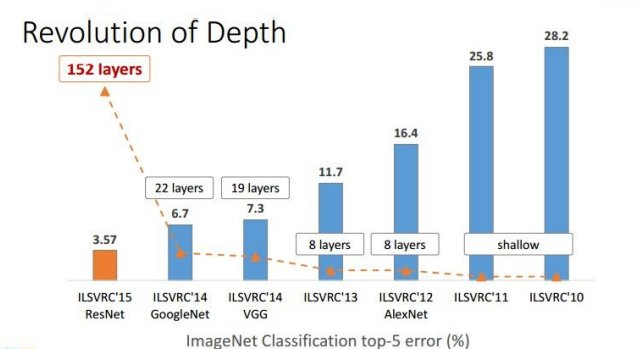
\includegraphics[width=0.4\textwidth]{ImageNet.png}}
\begin{figure}[t]
    \centering
    \caption{Comparison of errors in different architectures}
    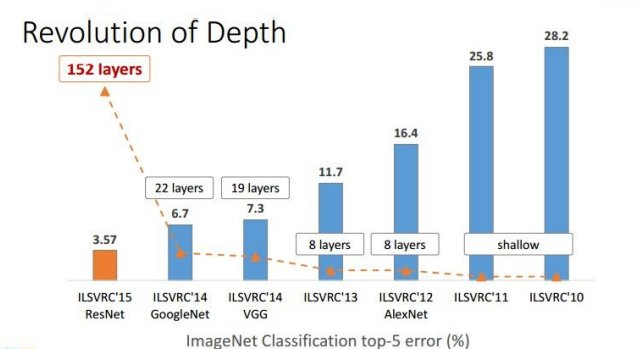
\includegraphics[width=1\textwidth]{ImageNet.png}
    %\caption*{Fonte: Autoria própria.} %% isso é levemente uma gambiarra, mas funciona para o propósito desse template.
    \label{fig:exemplo}
\end{figure}
So, in short:
\begin{itemize}
    \item A ConvNet has stacks of CONV, POOL, FC layers
    \item Trend towards smaller filter and deeper architectures
    \item Trend towards getting rid of POOL/FC layers (just CONV)
    \item A Typical architecture looks like $[(CONV-RELU)*N-POOL?]*M-(FC-RELU)*K,SOFTMAX$, where $N$ is  usually up to \~5, $M$ is large, $0 \leq K \leq 2$. But, recent advances such as ResNet/GoogLeNet challenge this paradigm

\end{itemize}

\section{Lecture 8 : Spatial Localization and Detection}
Some important Computer Vision tasks are:
\begin{itemize}
    \item Classification (single object)
    \item Classification $+$ Localization (single object)
    \item Object Detection (multiple objects)
    \item Instance Segmentation (multiple objects)
\end{itemize}
We look into Classification $+$ Localization and Object detection in this section using CNN.
\subsection{Classification $+$ Localization}

\subsubsection{Task}
%% para citar no texto, use \textcite{citacao} para ficar no formato Fulano (Ano), ou use \cite{citacao} para citar  no formato (FULANO, Ano)
\begin{itemize}
    \item \textbf{Classification} C classes, Input: Image, Output: Class label, Evaluation metric: Accuracy. It is basically classifying the object in the image that the image contains which object.
    \item \textbf{Localization} It means finding the coordinates or position of the object in image and boxing it. Input: Image, Output: Box in the image (x, y, w, h), Evaluation metric: Intersection over Union
    \item \textbf{Classification $+$ Localization} Doing both tasks together
\end{itemize}

\subsubsection{ImageNet}
Dataset consists of 1000 classes (same as classification) with each image having 1 class and at least 1 bounding box. There are \~800 training images per class. The algorithm produces 5 guesses of type (class, box). The example is correct if at least one guess among the ones produced by algorithm has correct class and bounding box (with at least 0.5 intersection over union).

\subsubsection{Idea \#1: Localization as Regression}
\begin{center}
    {\small Input Image $\xrightarrow{Neural Net}$ Output \& Correct Output: Box coordinates $\xrightarrow{}$ Loss: L2 distance}
\end{center}
Steps for classification $+$ localization as regression:
\begin{enumerate}
    \item Train or download a classification model, for example, AlexNet, VGG, GoogLeNet etc. This will do Convolution and pooling on the input image volume, then output will pass through Fully-connected layers, and you will get class scores.
    \item Attach a new fully-connected ``regression head" to the network. So, after getting final Conv feature map, it passes through FC layers giving class scores as ``Classification head" as well as FC layers giving Box coordinates as ``Regression head"
    \item Train the regression head only with SGD and L2 loss. That is, calculate the L2 loss from the Bos coordinates output.
    \item Use both the heads at test time.
\end{enumerate} 
For classification over $C$ classes, the classification head will give $C$ numbers (one per class) and the Class agnostic will give $4$ numbers (for one box), resulting in total $4 \times C$ numbers specific to a class (one box per class). The regression heads like DeepPose, R-CNN are attached after FC layer and those like Overfeat, VGG are attached after Conv layers. For localizing $K$ objects in each image, $4 \times K$ numbers will be produced (one box per object) for each image. For Human Pose estimation, we can represent a person by $K$ joints and regress (x,y) for each joint from last FC layer of AlexNet.

\subsubsection{Idea \#2: Sliding Window}
\begin{enumerate}
    \item It includes running classification $+$ regression network at multiple locations on a high-resolution image
    \item Then convert FC layers into Conv layers for efficient computation
    \item Now combine classifier and regressor predictions acorss all scales for final prediction
    \item At last we get the classification score for the object we were classifying. In practice, we use many sliding window locations and multiple scales.
\end{enumerate}
For localization, models like ResNet with deeper features come out to be more accurate and have less error (top 5).
\subsection{Object Detection}
For detecting many objects in a image, we need variable sized outputs as there will be many coordinates of each object when we consider detection as regression. If we consider detection as classification, we get output as Yes or no for a object classification and we need to test many positions and scaled, and use a computationally demandung classifier (CNN) for accurate results. The solution for this is to look at tiny subset of possible positions of objects. Putting it together, we achieve it by technique called \textbf{R-CNN}.

\subsubsection{R-CNN}
\begin{enumerate}
    \item First train or download a classification model, like AlexNet.
    \item Now Fine-tune the model for detection, that is:
    \begin{itemize}
        \item we need 20 object classes $+$ background instead of 1000 ImageNet classes
        \item Remove final FC layer and reinitialize from scratch
        \item Keep training the model using +ve or -ve regions from detection images
    \end{itemize}
    \item Extract features:
    \begin{itemize}
        \item get region proposals for all images
        \item for every region, warp to CNN input size, run forward through CNN, save pool5 feature
        \item you will need a big hard drive: \~200 GB for PASCAL dataset
    \end{itemize}
    \item Train 1 binary SVM per class to classify region features
    \item bbox regression: for every class, train a linear regression model to map the identified features to offsets to GT boxes. This will make up for ``slightly wrong" proposals
    \item For evaluation, we use a \textit{Mean Average Precision(mAP)} metric, which includes computing average precision separately for each class, then average over classes.
\end{enumerate}
So, R-CNN includes selective search with CNN classification or regression, but it is slow at test-time. For overcoming this problem there are other methods like \textbf{Fast R-CNN}: Swapping order of convolutions and region extraction or \textbf{Faster R-CNN}: Compute region proposals within the network, or another method called \textbf{YOLO}. It stands for \textit{You Only Look Once} for Detection as regression. It divides image into $S \times S$ grid and within each grid cell, it predicts $B$ boxes: 4 coordinates $+$ confidence and $C$ class scores. Then a regression from image to a $7 \times 7 \times (5*B + C)$ tensor. It uses direct prediction using a CNN and is even faster than Faster R-CNN, but not as good! For object detection also, deeper networks show better results.

\section{Lecture 9 : Understanding and Visualizing CNN}
\begin{itemize}
    \item Visualize patches that maximally activate neurons and their weights. Simplest way to understand them is to look at raw activations of CovNet. We can analyze it by picking any neuron and pick lots of images through CovNet and see which one excites that neuron the most. Another way is to look at the raw weights of filters. But, this can be done only on the first layer as it is the only one which has contact with input image. We can still do for other higher layers but that does not make much sense, they give gabor-like filters fatigue.
    \item Visualize the representation space (e.g. with t-SNE). The fc7 layer has 4096-dimensional ``code'' for an image. We can collect these codes for many images and use methods like t-SNE visualization to view them. t-SNE is a technique which embeds high-dimensional points so that locally, pairwise distances are conserved. In simple words, similar things end up in similar places, while dissimilar things end up wherever. So, two images whose CNN codes are close are placed nearby.
    \item Occlusion experiments - We slide over the image and output a classifier with probability of correct class, as a function of the position of the square of zeroes in original image. The regions with higher probability are more blue, and this indicates that the ConvNet was looking at this region for the object in the image
    \item Human experiment comparisons 
    \item Deconv approaches (single backward pass). It is about how to compute gradient of any arbitary neuron in the network with respect to image. The approach is as follows - 
    \begin{enumerate}
        \item Feed the image into ConvNet
        \item Pick a layer and set gradient there to be all 0 except 1 for a neuron of interest
        \item Backprop to image. But it won't be much interpretable, so we do ``Guided Backpropagation'' instead, which is based on the top 10 image patches activating this filter taken from ImageNet dataset.
    \end{enumerate}
     \item Optimization over image approaches (optimization) - It is about finding an image that maximizes some class score, that is $arg(max_{I} S_{C}(I) - \lambda ||I||_{2}^{2})$. The way we do this is:
     \begin{enumerate}
         \item Feed in zero image
         \item Set gradient of scores vector to be [0,0,..1,..0], then backprop to image.
         \item Do a small ``image update''
         \item Forward the image through the network, and go back to step 2.
     \end{enumerate}
\end{itemize}
For understanding ConvNets, Backpropping to the image is a powerful tool. It can be used for visualizing optimal stimuli for arbitrary neurons as well as segmenting object in the image. Also it helps in understanding Inverting codes, introducing privacy concerns, and adversarial examples.

\section{Lecture 10 : Recurrent Neural Networks}
RNN offers a lot of flexibility as they apply over sequences:
\begin{enumerate}
    \item one to one - Vanilla Neural Networks
    \item one to many - \textbf{Image Captioning}, image $\xrightarrow{}$ sequence of words!!
    \item many to one - Sentiment Classification, sequence of words $\xrightarrow{}$ sentiment
    \item many to many - Machine Translation, sequence of words $\xrightarrow{}$ sequence of words
    \item many to many - Video classification on frame level
\end{enumerate}
A RNN has a state of its own and it receives an input vectors through time. It modifies its state on basis of what it receives and usually wants to predict a vector at some time steps. 
\begin{equation*}
    x \xrightarrow[]{} RNN_\circlearrowleft \xrightarrow[]{} y
\end{equation*}
Let $x_i$ denote the input vectors and $h_t$ be the state. We process a sequence of vectors $x$ by applying a recurrence formula at every time step:
\begin{equation*}
    h_t = f_{W}(h_{t-1},x_t)
\end{equation*}
where, $h_t$ is new state, $f_W$ is some function with parameters $W$, $h_{t-1}$ is old state and $x_t$ is input vector at some time step. Notice that the same function with same set of parameters is applied for every time step $t$.
\subsection{RNN (Vanilla)}
The state consists of a single ``hidden'' vector $h$. A simple recurrence function is used here:
\begin{equation*}
  h_t = tanh(W_{hh}h_{t-1} + W_{xh}x_t)  \implies y_t = W_{hy}h_t
\end{equation*}
We can build a Character-level language model using RNN. We feed a sequence of characters into the neural network and at every single time step, we train the neural network to predict the next character in the character sequence. This type of model build using RNN by the professor is given \href{https://gist.github.com/karpathy/d4dee566867f8291f086}{here}. The code includes Loff function of 2 types - forward pass (compute loss) and backward pass (compute parameter gradient). Through this we can pass into a bunch of text into RNN and let it predict some meaningful text out of the sequence provided. At first it predicts something, may not be correct but then we train more and more by which the network learns and refines itself, thus finally some meaningful output. Sometimes the output from RNN sounds funny also, for example when it tried to learn mathematics proofs. It can also be used for searching for interpretable cells.

\subsection{Image Captioning}
Ah! this is the topic of project as well :) \\
We can use RNN for describing a image with sequence of words, which is called Image Captioning. It consists of 2 modules, there is a \textbf{CNN} for processing of the image and then there is a \textbf{RNN} as it is very good for modelling sequences.
\begin{enumerate}
    \item We take the test image and plug it into a CNN
    \item Normally at the end, we have a softmax classifier. But, here we get rid of it, anf redirect the image into a RNN.
    \item We plugin a ``start'' vector (300 dimensional) into RNN. It is a special starting vector which tells the RNN about the beginning of the sequence.
    \item Now we apply the recurrence formula, in which we also incorporate a third term, indicating the top of ConvNet also:
    \begin{equation*}
        h = tanh(Wxh * x + Whh * h + Wih * v)
    \end{equation*}
    \item The first output $y_0$ which we get from RNN, we plug it again into RNN with second state $h_1$ now, giving us $y_1$, and then repeat this process again and again to predict the next letters
    \item We sample this repeatedly until we sample a special ``end'' token, which tells us that RNN is now non-generating and it shows the end of sentence.
\end{enumerate}
The number of dimensions of this $y$ vector is the number of words in the vocabulary $+$ 1 for end token. \\
So, Vanilla RNNs are simple but they are not that great for work, it is common to use LSTM or GRU as their additive interactions imporove gradient flow. We can stack RNN together for more complex stuff:
\begin{equation*}
    h_{t}^{l} = tanh \, W^{l} \begin{pmatrix}
  h_{t}^{l-1} \\ 
  h_{t-1}^l 
\end{pmatrix}
\end{equation*}
where $h \in \mathbf{R}^n$ and $W^{l}[n \times 2n]$ \\ 
Apart from stacking, another way of making complex RNN is by using a better recurrence formula called \textbf{LSTM} - Long Short Term Memory:
\begin{equation*}
    \begin{pmatrix}
  i \\ f \\ o \\ g 
\end{pmatrix} =
\begin{pmatrix}
  sigm \\ sigm \\ sigm \\ tanh 
\end{pmatrix} W^{l}
\begin{pmatrix}
  h_{t}^{l-1} \\ 
  h_{t-1}^l 
\end{pmatrix}
\end{equation*}
\begin{equation*}
    c_{t}^l = f \odot c_{t-1}^l + i \odot g
\end{equation*}
\begin{equation*}
    h_{t}^l = o \odot tanh(c_{t}^l)
\end{equation*}
\begin{equation*}
    W^{l} [4n \times 2n]
\end{equation*}
It is just a complex recurrence function which is more useful and correct. Backward flow of gradients in RNN can explode or vanish but LSTM can control its vanishing and exploding is controlled with gradient clipping.
%%% as referências devem estar em formato bibTeX no arquivo referencias.bib

\printbibliography

\end{document}